\documentclass{sigchi}
\usepackage[hyphens]{url}
%\usepackage{hyperref}
%\hypersetup{breaklinks=true}

% Use this command to override the default ACM copyright statement (e.g. for preprints). 
% Consult the conference website for the camera-ready copyright statement.


%% EXAMPLE BEGIN -- HOW TO OVERRIDE THE DEFAULT COPYRIGHT STRIP -- (July 22, 2013 - Paul Baumann)
 \toappear{\scriptsize Permission to make digital or hard copies of all or part of this work for personal or classroom use is granted without fee provided that copies are not made or distributed for profit or commercial advantage and that copies bear this notice and the full citation on the first page. Copyrights for components of this work owned by others than ACM must be honored. Abstracting with credit is permitted. To copy otherwise, or republish, to post on servers or to redistribute to lists, requires prior specific permission and/or a fee. Request permissions from permissions@acm.org. \\
{\emph{CHI 2015}}, April 18 - 23 2015, Seoul, Republic of Korea.\\
Copyright is held by the owner/author(s). Publication rights licensed to ACM.\\
ACM 978-1-4503-3145-6/15/04...\$15.00.\\
http://dx.doi.org/10.1145/2702123.2702164}
%% EXAMPLE END -- HOW TO OVERRIDE THE DEFAULT COPYRIGHT STRIP -- (July 22, 2013 - Paul Baumann)


% Arabic page numbers for submission. 
% Remove this line to eliminate page numbers for the camera ready copy
% \pagenumbering{arabic}


% Load basic packages
\usepackage{balance}  % to better equalize the last page
\usepackage{graphicx} % for EPS, load graphicx instead
\usepackage{times}    % comment if you want LaTeX's default font
\usepackage{url}      % llt: nicely formatted URLs
\usepackage{multirow} % http://ctan.org/pkg/multirow
\usepackage{tabu}
\usepackage{pgfplots}
\graphicspath{ }

% llt: Define a global style for URLs, rather that the default one
\makeatletter
\def\url@leostyle{%
  \@ifundefined{selectfont}{\def\UrlFont{\sf}}{\def\UrlFont{\small\bf\ttfamily}}}
\makeatother
\urlstyle{leo}


% To make various LaTeX processors do the right thing with page size.
\def\pprw{8.5in}
\def\pprh{11in}
\special{papersize=\pprw,\pprh}
\setlength{\paperwidth}{\pprw}
\setlength{\paperheight}{\pprh}
\setlength{\pdfpagewidth}{\pprw}
\setlength{\pdfpageheight}{\pprh}

% Make sure hyperref comes last of your loaded packages, 
% to give it a fighting chance of not being over-written, 
% since its job is to redefine many LaTeX commands.
\usepackage[pdftex]{hyperref}
\hypersetup{
pdftitle={SIGCHI Conference Proceedings Format},
pdfauthor={LaTeX},
pdfkeywords={SIGCHI, proceedings, archival format},
bookmarksnumbered,
pdfstartview={FitH},
colorlinks,
citecolor=black,
filecolor=black,
linkcolor=black,
urlcolor=black,
breaklinks=true,
}

\def\etal{{\it et al.~}}

\newenvironment{packed_enum}{
\begin{enumerate}
  \setlength{\itemsep}{1pt}
  \setlength{\parskip}{0pt}
  \setlength{\parsep}{0pt}
}{\end{enumerate}}


\newenvironment{packed_item}{
\begin{itemize}
  \setlength{\itemsep}{1pt}
  \setlength{\parskip}{0pt}
  \setlength{\parsep}{0pt}
}{\end{itemize}}


% create a shortcut to typeset table headings
\newcommand\tabhead[1]{\small\textbf{#1}}


% End of preamble. Here it comes the document.
\begin{document}

\title{Somebody's Watching Me?}
\subtitle{Assessing the Effectiveness of Webcam Indicator Lights}

\numberofauthors{1}
\author{
 \alignauthor Rebecca S. Portnoff\textsuperscript{1}, Linda N. Lee\textsuperscript{1},\\Serge Egelman\textsuperscript{1,2}, Pratyush Mishra\textsuperscript{1}, Derek Leung\textsuperscript{1}, and David Wagner\textsuperscript{1}\\
   \vspace{0.5em}
   \affaddr{\textsuperscript{1}University of California, Berkeley, CA\\ \{rsportnoff,lnl,egelman\}@cs.berkeley.edu, \{pratyushmishra,derek.leung\}@berkeley.edu}\\ 
   \affaddr{\textsuperscript{2}International Computer Science Institute, Berkeley, CA, egelman@icsi.berkeley.edu}\\
}

%\numberofauthors{6}
%\author{
%  \alignauthor Rebecca Portnoff\\
%    \affaddr{Affiliation}\\
%    \affaddr{Address}\\
%    \email{e-mail address}\\
%    \affaddr{Optional phone number}
%  \alignauthor Linda N. Lee\\
%    \affaddr{Affiliation}\\
%    \affaddr{Address}\\
%    \email{e-mail address}\\
%    \affaddr{Optional phone number}    
%  \alignauthor Serge Egelman\\
%    \affaddr{Affiliation}\\
%    \affaddr{Address}\\
%    \email{e-mail address}\\
%    \affaddr{Optional phone number}
%  \alignauthor Derek Leung\\
%    \affaddr{Affiliation}\\
%    \affaddr{Address}\\
%    \email{e-mail address}\\
%    \affaddr{Optional phone number}
%  \alignauthor Pratyush Mishra\\
%    \affaddr{Affiliation}\\
%    \affaddr{Address}\\
%    \email{e-mail address}\\
%    \affaddr{Optional phone number}
%  \alignauthor David Wagner\\
%    \affaddr{Affiliation}\\
%    \affaddr{Address}\\
%    \email{e-mail address}\\
%    \affaddr{Optional phone number}
%}

\maketitle

\begin{abstract}
Most laptops and personal computers have webcams with LED indicators to notify users when they are recording. Because hackers use surreptitiously captured webcam recordings to extort users, we explored the effectiveness of these indicators under varying circumstances and how they could be improved.  We observed that, on average, fewer than half of our participants (45\%) noticed the existing indicator during computer-based tasks.  When seated in front of the computer performing a paper-based task, only 5\% noticed the indicator.  We performed a followup experiment to evaluate a new indicator and observed that adding onscreen glyphs had a significant impact on both computer-based and non-computer-based tasks (93\% and 59\% noticed the new indicator, respectively).  We discuss how our results can be integrated into current systems, as well as future ubiquitous computing systems.
\end{abstract}

\keywords{Privacy Indicators; Ubiquitous Computing; Usable Security}

\category{K.6.5.}{Management of Computing and Information Systems}{Security and protection}
\category{H.5.2.}{Information Interfaces and Presentation (e.g. HCI)}{User Interfaces}

\section{Introduction}

As we enter the age of wearable and ubiquitous computing, more and more consumer computing devices will accept continuous input via audio and/or video sensors.  These devices allow applications to perform a wide range of actions, from recognizing objects in the user's environment to parsing voice commands.  Similar to smartphone platforms~\cite{Felt2011}, ubiquitous computing platforms will need permission mechanisms to allow users to regulate {\it how} specific applications access sensitive data, and privacy indicators to communicate {\it when} that data is accessed. In order for us to understand the design space of these privacy indicators, we examined the effectiveness of similar privacy indicators that are already sufficiently pervasive: webcam recording indicators.

For several years now, laptop sales have surpassed desktop sales~\cite{Eddy2008}, and with few exceptions, it is standard for a new laptop to come equipped with a built-in webcam.  These webcams face the user and have indicator LEDs to communicate when the webcam is recording. Ideally, the user will notice the indicator, understand that a recording is being made, and take defensive actions in the event that the webcam is recording without the user's consent. Anecdotal evidence suggests that these assumptions are incorrect~\cite{Checkpoint2013}.

Remote Administration Tools (RATs) allow hackers to control an unsuspecting user's computer remotely, allowing them to execute programs, send taunting messages, or eavesdrop via the webcam and microphone~\cite{Anderson2013}.  In some cases, hackers have used videos of victims in various states of undress as part of ``sextortion'' plots: the perpetrator threatens to publicly post the captured videos and/or photos unless the victim pays a ransom~\cite{Anderson2011}. The most famous case of this involved a high school classmate of Miss Teen USA who surreptitiously captured photos of her naked in her bedroom~\cite{Dobuzinskis2013}.  Unauthorized access to laptop webcams is not just limited to extortionists, however.  In 2010, the Lower Merion School District in Pennsylvania paid a settlement to victims after it was reported that school administrators were spying on students in their homes using school-provided laptops~\cite{Hill2010}.
 
While users can buy stickers to cover up the webcams to prevent unauthorized video capture~\cite{EFFSticker}, we wanted to explore the effectiveness of current webcam LED indicators and examine ways in which they could be improved, so that our findings can be applied to future technologies.  We performed a series of experiments to quantify how often users are likely to take notice when their webcams unexpectedly turn on.  First, we turned on the webcam unexpectedly while participants were using the computer, to see how often they noticed and whether this was affected by their activities.  Next, we studied the effectiveness of a new indicator.  In this work, we contribute the following:

\begin{packed_item}
\item We show that in our laboratory environment, a minority of participants (45\%) noticed an illuminated webcam LED indicator when performing a computer-based task, regardless of what that task specifically was.  When performing tasks not on the computer, but in its proximity, only 5\% of participants noticed the webcam LED.
\item We show that the use of full-screen glyphs significantly increases the likelihood that participants notice the webcam indicator: both when performing computer-based tasks (93\%) and non-computer-based tasks (59\%).
\end{packed_item}

%In what follows, we present related work, responses from an initial online survey, and the results of two laboratory experiments. We then interpret the responses to our exit survey, discuss future mitigation research, and state our conclusions.

\section{Related Work}

%We examined the effectiveness of webcam LEDs, in terms of whether they are noticeable and understandable.
In this section, we present related work on webcam indicator attacks, privacy/security indicator design and evaluation, and privacy considerations for ubiquitous computing.

\subsection{Attacks on Webcam LEDs}
In order for users to notice and comprehend privacy indicators, they must be reliably present. Although our work assumes that webcam LEDs will reliably illuminate when a recording is being made, recent studies demonstrate that this assumption is not always correct. Most webcam LEDs are wired in the same logical connection as the webcam, so that the LED will turn on with the webcam. This varies from device to device, however, with some indicators controlled by software~\cite{LogitechAnswer}. Nevertheless, because of this, many people incorrectly believe that it is not possible to disable the indicator without attacking the hardware. 

Recent research, however, shows that an attacker can exploit software vulnerabilities to cause some of these indicators to malfunction. Broker \etal demonstrated an attack on webcam firmware that enables video capture without turning on the webcam LED on older versions of Mac laptops~\cite{iSight}. While these attacks are troubling, we assume that devices will eventually be designed so that indicators cannot be disabled; research on understanding whether the indicators are effective at communicating risk to users is still necessary.

\subsection{Indicators and Warnings}
Cranor discusses various evaluation criteria for indicators and warnings~\cite{cranor2006they}, such as how an indicator interacts with other indicators, and whether users notice, understand, and follow its recommendations, both after first exposure and then repeated exposures. Other considerations include how warnings are displayed~\cite{egelman2008you}, when they are displayed~\cite{egelman2009timing}, and how they make use of icons and signal words~\cite{amer2007signal}. 

Poorly designed indicators not only fail to communicate the appropriate message to users, but can have other unintended negative consequences, such as desensitization, habituation, or  annoyance~\cite{stewart1994intended}. They can also create a false sense of security~\cite{cannella2004secure}. For example, when people notice the HTTPS lock icon (and they tend not to~\cite{whalen2005gathering}) they often incorrectly assume that it indicates a secure website, rather than a secure connection~\cite{Friedman2002}.  Users also do not change their behavior when this indicator is absent~\cite{schechter2007emperor}. When designing privacy and security indicators, it is important to examine these potential pitfalls.
 
 \subsection{Privacy Concerns for Ubiquitous Sensing} 
Wearable devices and ubiquitous sensing platforms are moving towards automated capture and access~\cite{abowd2000charting}. More and more often, people will interact with sensors while carrying out daily activities, from a myriad of sources and for a variety of reasons: ``lifelogging'' devices to record their daily lives~\cite{hoyle2014privacy,dickie2004augmenting}, memory augmentation devices~\cite{chen2010augmenting,devaul2003memory,kalnikaite2010now}, smart homes that optimize living conditions~\cite{chan2008review,chan2009smart,edwards2001home}, devices that create augmented reality environments~\cite{azuma1997survey,azuma2001recent}, and even devices integrated into clothing \cite{anliker2001weararm}.
 
The ubiquitous capture and storage of information naturally raises concerns about the preservation of privacy~\cite{palen2003unpacking}. Privacy in the field of ubiquitous computing relies on principles including notice, choice, and consent~\cite{langheinrich2001privacy}. Certain privacy problems stem from poor feedback mechanisms~\cite{bellotti1993design,dourish2004security}: indicators failing to reliably inform people {\it when} they are being captured and {\it what} information is being saved. 

Clearly, there is a critical need for effective privacy indicators that users will notice and understand. Research has suggested that notifications in a user's peripheral field of vision may be acceptable for certain cases~\cite{costanza2006eye}. It is not clear, however, whether this is an effective strategy for every or even most privacy and security notifications. 

Although significant work has been done to explore privacy/security indicator designs, researchers have not yet focused specific attention on the ubiquitous webcam LED.

%In the following section, we begin this work by outlining the responses from our online survey exploring peoples' understanding of webcam security.

\section{Awareness and Perceptions}
To quantify the problem of ``webcam spying,'' we first conducted an online survey. Our goal was to better understand whether people are likely to be at risk, their awareness of the danger, and how many claim to have already been victimized.

\subsection{Methodology}
We recruited 500 participants on December 9th, 2013 via Amazon's Mechanical Turk. We restricted participants to those over 18 years old residing in the U.S. All participants stated that they owned a laptop or desktop computer with either an external or internal webcam. We asked questions about participants' webcam use and their understanding of the indicator LED. The questions fell into three categories:

\begin{packed_enum}
\item {\it Behavior}: The types of participants' webcams and whether they obscure them when not in use.
\item {\it Risk Awareness}: Whether participants believe that webcam spying is possible.
\item {\it Victimization}: Whether participants have noticed the webcam LED previously come on against their wishes.
\end{packed_enum}

The entire survey took approximately 7 minutes to complete, upon which we compensated them \$1.

\subsection{Results}
After removing 8 incomplete responses, our sample consisted of 492 participants (64\% male and a median age range of 26-30). Two researchers independently coded 1,476 open-ended responses (94.3\% agreement), discussed any disagreements, and resolved them to reflect unanimous agreement.

%\begin {table}
%\centering
%\begin{tabular}{lll}
%             & Computer Task & Non-Computer Task \\
%\hline
%would notice & 72.3\% (357 of 494) & 29.8\% (148 of 497) \\
%would not notice & 14.4\% (71 of 494) &  42.3\% (210 of 497) \\
%not sure & 13.4\% (66 of 494) & 28.0\% (139 of 497) \\
%\hline
%\end{tabular}
%\caption {Perception of Noticing the LED light: MTurk Responses}
%\end {table}

\subsubsection{Behavior}

We asked laptop-owning participants whether they ``always,'' ``sometimes,'' or ``never'' close their laptop lids when not using it. We found that 45\% reported ``always'' doing so, whereas another 36\% reported doing so ``sometimes.'' We also asked whether participants were comfortable doing any of the following in front of an open laptop:

\begin{packed_item}
\item Going to the restroom
\item Eating meals
\item Changing clothes
\item Talking to friends
\item Taking a shower
\end{packed_item}

We found that 28\% were comfortable using the restroom, 85\% were comfortable eating meals, 41\% were comfortable changing clothes, 80\% were comfortable talking to a friend, and 18\% were comfortable taking a shower. Because we previously subjected participants to questions regarding webcams before answering this question, these numbers are likely under-reported and therefore represent lower bounds.
While we are not aware of any peer-reviewed literature on the matter, an industry-commissioned survey reports that 44\% of respondents use their laptops in the bedroom and 8\% in the bathroom~\cite{RouseSomeone}. Our data suggests that large groups of users practice behavior that puts them at risk of webcam spying.

\subsubsection{Risk Awareness}

We asked participants whether they thought it would be possible for a hacker to spy on them through their webcam, and to indicate why or why not. We found that 13\% did not think it would be possible, and 19\% were unsure. The open-ended responses ranged in technical fluency, ranging from distrust of the notion of foolproof technologies to discussing how root access could allow an attacker to control a device. 

\subsubsection{Victimization}
%(3.9\% of 492) 
Nineteen participants reported that their webcam LED turned on when they were not using it. Almost all of them (18 of 19) believed this was normal behavior or just due to human error, while one participant was the victim of ransomware, stating: 

\begin{quotation}
\noindent {\it ``I had contracted a virus on my laptop the FBI classifies as `ransomware.' It tells you you cannot access your computer unless you wire money to an account, and it turns on the webcam to frighten people. I was surprised and very anxious, and I responded by covering my webcam with black electrical tape.''} (P30)\\
\end{quotation}

Our survey showed that many people practice habits that increase their risk and that they are unaware of the danger. In the following section, we describe our empirical evaluation of the common webcam LED, in terms of the proportion of users who are likely to notice it when it unexpectedly illuminates, and whether this varies based on the task being performed. 

\section{Laboratory Experiment}

We conducted a laboratory experiment to examine the extent to which people notice and understand current webcam LEDs, as well as the extent to which their activities impact the likelihood of noticing the LEDs. We explored this because an attacker with remote access to a victim's webcam would also be able to see what the victim is doing, and potentially use this information to increase attack effectiveness. In this section, we provide details of our methodology and results.

\subsection{Methodology}
We conducted an experiment with 98 participants.  All participants used Toshiba Tecra R850 laptops, which use a blue LED next to the webcam lens to indicate when the webcam is recording. We examined whether participants noticed the webcam LED turning on when performing a computer-based task, as well as a non-computer-based task within close proximity of the webcam (i.e., answering a written questionnaire). %We describe our procedure and recruiting method.

\subsubsection{Procedure}
We conducted each session in a laboratory space at our university that consisted of 36 laptops, in 6 rows, with cubicle walls separating each laptop. No more than 15 participants attended each session. We distanced each participant from every other participant by at least one desk, by only using every other laptop in each staggered row. Our goal was to prevent participants from viewing each other's laptops.

Upon arriving, participants sat down at laptops of their choosing, where consent forms were present. Once participants read and signed the consent forms, the researcher outlined participants' tasks and explained that the purpose of the study was to see how people perform various tasks on a computer. Again, the true purpose of the study was not revealed. Each session proceeded as follows:

\begin{packed_enum}
\item Participants answered the 30-item Barratt Impulsiveness Scale~\cite{Patton1995}, which was used as a distraction to make them comfortable with the environment.
\item Participants performed one of four randomly-assigned computer-based tasks lasting 10-15 minutes. At some random point after 5 minutes, the webcam made a 10 second recording. Participants were prevented from advancing to the next task until at least 10 minutes had elapsed. There were four different types of computer-based tasks:
\begin{packed_item}
\item {\bf Reading}: Participants read a provided passage~\cite{Filkins2014}. We told them that they would be asked questions about the reading, so they should read it thoroughly.
\item {\bf Essay}: Participants saw a previous year's SAT writing prompt. We told them to write an essay based on the prompt as part of a college or job application.
\item {\bf Game}: Participants played the 2048 game.\footnote{http://gabrielecirulli.github.io/2048/} We instructed them to try to get as high a score as possible in 10-15 minutes.
\item {\bf Video}: Participants watched a TED talk,\footnote{https://www.youtube.com/embed/xMj\_P\_6H69g} which we told them they would be asked questions about.
\end{packed_item}
\item Each participant took the Cognitive Reflection Test on a printed sheet of paper on the desk in front of the laptop~\cite{Frederick2005}. At some random point after 60 seconds into the task, the webcam made a 10 second recording. Participants were prevented from advancing to the exit survey until at least 2 minutes had elapsed.
\item Each participant filled out an exit survey on the computer. 

%SE: We should put this in the exit survey section; there's no need to mention details here, since we'll just need to repeat them when presenting the data.

%Our questions fell into the following categories:
%\begin{packed_item}
%\item {\it Noticing the indicator (unprompted)}: We asked participants to describe whether anything unexpected occurred during the computer-based task or during the written questionnaire. Responses were open-ended. The purpose of these questions was to examine whether participants would report the indicator turning on, without being prompted.
%\item {\it Noticing the indicator (prompted)}: Next, we explicitly asked participants whether any of the given multiple-choice options had occurred on the computer during the computer-based task, and then during the written questionnaire. The purpose of these questions was to discover how many participants reported noticing the indicator, after prompting them.
%\item {\it Prior experiences}: We asked participants whether they, or anyone they knew, had ever noticed the webcam on their home computer or laptop turn on unexpectedly. They described any actions they took, and any consequences they experienced. The purpose of these questions was to determine whether previously experiencing their personal webcam turn on unexpectedly correlated with participants noticing the indicator in the laboratory experiment.
%\item {\it Risk Perceptions and Security/Privacy Concerns}: We asked participants to describe any thing that might cause the webcam on their home computer or laptop to begin recording unexpectedly. We also asked them to describe any potential consequences if they were unexpectedly recorded via their computer webcam in their own home, and the video became public. The purpose of these questions was to determine whether participants who noticed the webcam LED had more concerns, or a higher sense of potential risks and problems.
%\item {\it Security Behavior}: We asked participants whether they covered their camera lens with any kind of tape or occluding material. We also asked participants to describe what they would do if the webcam on their home computer/laptop began recording unexpectedly. The purpose of these questions was to determine whether participants who practiced safer security behavior were more likely to notice the webcam LED light in the laboratory experiment.
%\end{packed_item}
\item Upon completing the exit survey, we debriefed participants. We gave each participant a re-consent form, which would allow us to use the webcam video in our analysis, and paid them with \$35 debit cards.
\end{packed_enum}

%Two researchers independently read over all open-ended question responses to construct codebooks, after which they met to agree on the set of final codes for each question. After independently coding all responses, they met a final time to discuss these codings and resolve any disagreements.

\subsubsection{Recruitment}
We placed an online recruitment advertisement on Craigslist in June of 2014, under the ``writing/editing'' jobs section for our city and surrounding cities. The advertisement stated that the study was about how people perform various tasks on a laptop. Those interested in participating filled out an online screening survey in which they provided information about their age, gender, laptop make and model, amount of time using their laptop, various ways they have used their laptop (social networking, video recording, playing games, making video calls, making online purchases), contact information, and availability. We screened out those who were under 18 years of age or who had a laptop that did not have a webcam.

We recruited 98 participants who showed up for sessions lasting 30-60 minutes. Of our 98 participants, 55 were female (56\%), and ages ranged from 18 to 72 ($\mu = 37.9$, $\sigma = 15.4$).

\subsection{Results}
Our primary goal was to assess the effectiveness of the webcam LED. We found that the majority of participants did not notice it turn on during either task, and many did not understand what it indicated, even when they did notice it. In this section, we provide details for whether participants noticed the webcam LED, our efforts to corroborate the self-reports using the captured videos, whether any of the computer-based task conditions influenced the participants to notice the webcam LED more or less, and participants' understanding of the purpose of the webcam LED.

\subsubsection{Noticing the Indicator}
We determined whether participants noticed the webcam LED through multiple exit survey questions. First, we asked them if anything unexpected had occurred as they completed the computer-based task and the written task. We used open-ended formats so as to not prime them (i.e., we made no mention of the webcam). We accepted responses that reported the webcam or the LED turning on as evidence that they noticed it. Only 27.6\% (27 of 98) of participants reported noticing it during the computer-based task (Table \ref{unprompted}). No participants reported noticing the webcam LED during the written task.


\newcommand*{\MyIndent}{\hspace*{0.5cm}}%
\begin {table}
%\small
\centering
\begin{tabular}{lrl}
             & Noticed light & \\
\hline
\textbf{Computer Task} & 27.6\% & n = 98 \\
\MyIndent Reading & 46.4\% & n = 28 \\
\MyIndent Essay & 25.0\% &  n = 28 \\
\MyIndent Game & 25.0\% & n = 20\\
\MyIndent Video & 9.0\% & n = 22 \\
\textbf{Written Task} & 0\% & n = 98 \\
\hline
\end{tabular}
\caption {Unprompted responses: the number of participants who described noticing the webcam LED turn on during each task.}
\label{unprompted}
\end {table}

\begin {table}
%\small
\centering
\begin{tabular}{lrrl}
             & Light turned on & Recording \\
\hline
\textbf{Computer Task} & 44.9\% & 33.7\% & n = 98 \\
\MyIndent Reading & 53.6\% & 32.1\% & n = 28 \\
\MyIndent Essay & 35.7\% & 32.1\% & n = 28 \\
\MyIndent Game & 45.0\% & 30.0\% & n = 20 \\
\MyIndent Video & 45.5\% & 40.9\% & n = 22 \\
\textbf{Written Task} & 5.1\% & 5.1\% & n = 98 \\
%\MyIndent Reading & 3.6\% & 0\% & n = 28 \\
%\MyIndent Essay & 7.1\% & 10.7\% & n = 28 \\
%\MyIndent Game & 10.0\% & 5.0\% & n = 20 \\
%\MyIndent Video & 0\% & 4.5\% & n = 22 \\
\hline
\end{tabular}
\caption {Prompted responses: the number of participants who selected either that the webcam LED turned on or the webcam began recording.}
\label{prompted}
\end {table}

On the next page of the exit survey, we asked participants which (if any) of the following occurred during the computer-based task, and then during the written task. For each participant, we randomized the order of the following options:
\begin{packed_item}
\item The webcam began recording
\item A light above the screen turned on
\item The desktop background changed
\item An unexpected sound played
\item The screen flickered
\item The computer rebooted
\item None of the above
\end{packed_item}

Once prompted, the rate at which participants reported noticing the light increased. During the computer-based task it increased to 44.9\% (44 of 98), whereas during the written task, it increased from 0\% to 5.1\% (5 of 98).

%his difference between unprompted and prompted responses was statistically significant (\textit{p} $<$ 0.018; two-tailed), but with a very small effect size (Cramer's \textit{V} = 0.1804).

To corroborate our exit survey data, we examined the webcam recordings. Four of our 98 participants declined to give us permission to use their recordings. Three researchers independently coded all 188 recordings (two per participant) to judge whether each participant made eye contact with the camera (i.e., an indication that they were looking at it), and if so, at what point in time during the 10 second recording. The researchers then resolved any disagreements, so that final codings were unanimous. Prior to achieving consensus, they disagreed on 26 instances (86.2\% agreement).

Based on the recordings, 48.9\% (46 of 94) of participants noticed the webcam LED during the computer-based task, and 4.26\% (4 of 94) noticed it during the written task (Table \ref{eyecontact}). During the computer-based task, of the 46 participants who we observed making eye contact with the webcam, all of them did so within the first four seconds; 71.7\% (33 of 46) noticed it immediately (Figure \ref{eyehist}). During the written task, all four of them noticed within the first seven seconds.

Using our three different metrics (unprompted responses, prompted responses, and recordings), we concluded that 27\%-49\% of participants noticed the webcam LED during the computer-based task, whereas $\leq5\%$ noticed it during the written task. Since the recordings and prompted responses were similar, we did not consider the recordings further.

% at 0:
%R: 11, CT. 1, WQ.
%W: 8,  0
%G: 7, 0
%V: 7, 0
%2, 0, 1, 1
%Reading & 63.0\% & 7.41\% & n = 27 \\
%	& (17/27) & (11/27) & (10/18) & (8/22) \\
%Essay & 40.7\% &  0\% & n = 27 \\
%	& (16/27) & (16/27) & (8/18) & (14/22) \\
%Game & 55.6\% &  5.56\% & n = 18 \\
%Video & 36.4\% &  4.55\% & n = 22 \\
%Total & 48.9\% &  4.26\% & n = 94 \\

\begin {table}
%\small
\centering
\begin{tabular}{lrl}
             & Made Eye Contact & \\
\hline
\textbf{Computer Task} & 48.9\% & n = 94 \\
\MyIndent Reading & 63.0\% & n = 27 \\
\MyIndent Essay & 40.7\% & n = 27 \\
\MyIndent Game & 55.6\% & n = 18 \\
\MyIndent Video & 36.4\% & n = 22 \\
\textbf{Written Task} & 4.26\% & n = 94 \\
\hline
\end{tabular}
\caption {Participants observed making eye contact with the webcam.}
\label{eyecontact}
\end {table}

\begin{figure}
\centering
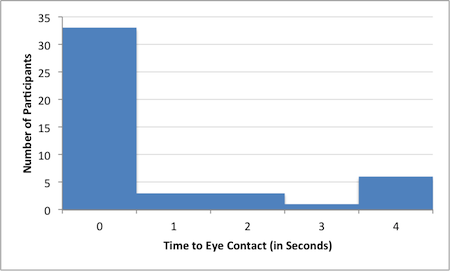
\includegraphics[height=0.2\textheight]{chart.png}
\caption{Time into recording at which participants made eye contact.}
\label{eyehist}
\end{figure}


%SE: This is hard to follow and I'm not sure adds much.
%Of those who made eye contact with the camera during the computer-based task, when prompted, the majority - 84.8\% (39 of 46) - reported either seeing the webcam LED or that the webcam began recording (see Table 5).  Making eye contact with the camera correlated with reporting noticing either the LED light turn on or that the webcam began recording during the exit survey (\textit{r} = 0.49, \textit{p} $<$ 0.0001) when prompted, for the computer-based task. For the written questionnaire, there was no correlation between eye contact and whether they reported it in the exit survey  (\textit{r} = 0.49, \textit{p} $=$ 1.0) when prompted. However, the number of people who noticed the LED during the written questionnaire is so small that we believe this is not a good test for correlation.



%This is compounded by the fact that, as we saw in our Amazon Mechanical Turk study, people believe they will notice the webcam light at a much higher rate than they actually do (see Table 1). More than 70\% of participants believed they would notice if the webcam LED turned on while using the computer for a task not directly related to the webcam - significantly more than the 44.9\% of participants who actually noticed in our in-person study. We saw the same difference when asking if participants would notice the webcam LED while in the same room as the webcam, but not working on the computer: almost 30\% believed they would, significantly more than the 5.1\% who actually noticed in our in-person study.

\subsubsection{Task Influence}

We examined the effects of participants' tasks on noticing the webcam LED. We analyzed differences between computer-based tasks and the written task (within-subjects), as well as between specific computer-based tasks (between-subjects).

We determined using McNemar's test that participants were significantly more likely to notice the indicators when performing the computer-based task, based on both the unprompted (\textit{p} $<$ 0.0001; $\chi^2$ = 25.037) and prompted (\textit{p} $<$ 0.0001; $\chi^2$ = 33.5814) responses.  Using either measure, we observed relatively large effect sizes (\textit{$\phi_{unprompted}$} = 0.505, \textit{$\phi_{prompted}$} = 0.585), which indicates that participants were more likely to notice the webcam LED while performing a task on the computer, rather than merely in its proximity.

When it came to differences between specific computer-based tasks, we did not observe statistically significant results when examining both unprompted ($\chi^2(3)=5.917$, $p<0.116$) and prompted ($\chi^2(3)=1.000$, $p<0.8013$) responses. Thus, we conclude that the specific computer-based tasks that we evaluated had no observable effect on whether participants noticed the indicator.


%When looking at each of the computer-based task conditions separately, we found that in all cases but when participants were unprompted during the computer-based tasks, we were unable to reject the null hypothesis that participants' computer-based tasks have no demonstrable impact on whether they noticed the indicators.

%When unprompted during the computer-based task (see Table 2), we were able to reject the null hypothesis (\textit{p} $<$ 0.0305; two-tailed) with (Cramer's \textit{V} = 0.3015). When unprompted during the written questionnaire, we were unable to reject the null hypothesis. We found that the computer-based tasks had no impact on whether they noticed the indicators: regardless of the task, none of the participants reported the LED turning on. 

%            & Reading & Essay & Game & Video \\
%LED & 46.4\%  & 25.0\% & 25.0\% & 9.0\% \\
%			& (13/28) & (7/28) & (5/20) & (2/22) \\
%nothing & 35.7\% & 35.7\% & 45.0\% & 63.6\%  \\
%			& (10/28) & (10/28) & (9/20) & (14/22) \\
%something else & 17.9\% & 39.2\% & 30.0\% & 27.3\% \\
%			& (5/28) & (11/28) & (6/20) & (6/22) \\
%\caption {Unprompted Responses By Computer-Task, during Computer-Task: Standard LED}
%13 15 p 0.0166 c 0.2673
%7 21 p 0.9203 c 0.0364
%5 15 p 1 c 0.0286
%2 20 p 0.0538 c 0.2222

%When prompted during the computer-based task (see Table 3), we were unable to reject the null hypothesis (\textit{p} $=$ 0.6128; two-tailed). The same was the case during the written questionnaire:  (\textit{p} $=$ 0.6128; two-tailed)

%            & Reading & Essay & Game & Video \\
%	&  n = 28 & n = 28 & n = 20 & n = 22 \\
%light & 53.6\%  & 35.7\% & 45.0\% & 45.5\% \\
%recording & 32.1\% & 32.1\% & 30.0\% & 40.9\%  \\
%light & 53.6\%  & 35.7\% & 45.0\% & 45.5\% \\
%			& (15/28) & (10/28) & (9/20) & (10/22) \\
%recording & 32.1\% & 32.1\% & 30.0\% & 40.9\%  \\
%			& (9/28) & (9/28) & (6/20) & (9/22) \\
%something else & 14.3\% & 14.3\% & 0\% & 9.1\% \\
%			& (4/28) & (4/28) & (0/20) & (2/22) \\
%nothing & 32.1\% & 46.4\% & 50.0\% & 40.9\% \\
%			& (9/28) & (13/28) & (10/20) & (9/22) \\
%\caption {Prompted Responses By Computer-Task, during Computer-Task: Standard LED}
%15 13 | 29 p 0.3865 c 0.1102
%10 18 | 34 p 0.351 c 0.1169
%9 11 | 35 43 p 0.8065 c 0
%10 12 | 34 42  p 0.8625 c 0

%            & Reading & Essay & Game & Video \\
%light & 3.6\%  & 7.1\% & 10.0\% & 0\% \\
%			& (1/28) & (2/28) & (2/20) & (0/22) \\
%recording & 0\% & 10.7\% & 5.0\% & 4.5\%  \\
%			& (0/28) & (3/28) & (1/20) & (1/22) \\
%something else & 7.1\% & 14.3\% & 0\% & 9.1\% \\
%			& (2/28) & (4/28) & (0/20) & (2/22) \\
%nothing & 89.3\% & 78.6\% & 90.0\% & 86.4\% \\
%			& (25/28) & (22/28) & (18/20) & (19/22) \\
%\caption {Prompted Responses By Computer-Task, during Written Questionnaire: Standard LED}
%1 27 | 29 p 0.3865 c 0.1102
%2 26 | 34 p 0.351 c 0.1169
%2 18 | 35 43 p 0.8065 c 0
%0 22 | 34 42  p 0.8625 c 0

%Given the lack of noticeable effect (among this sample size) based on task, for the mitigations we chose to %focus on just the video task, as it had the lowest rate for people noticing the LED light.


%Computer Task
%eye contact | yes light/recording , no light/recording: 39 , 7
% no eye contact | yes, no 12 , 36 Cramer's V 0.5999
%WQ
%eye contact | yes light/recording , no light/recording: 0 , 4
% no eye contact | yes, no 5, 43
%and reporting noticing the webcam begin recording (\textit{r} = 0.46, \textit{p} $<$ 0.0005). 
%LED light (\textit{r} = 0.49, \textit{p} $<$ 0.0005)

%light & 71.7\% (33 of 46) & 20.8\% (10 of 48) \\
%recording & 56.5\% (26 of 46) &  12.5\% (6 of 48) \\

%\begin {table}
%\small
%\centering
%\begin{tabular}{lll}
%             & light above screen & \\
%\hline
%%light & 71.7\% (33 of 46) & 20.8\% (10 of 48) \\
%%recording & 56.5\% (26 of 46) &  12.5\% (6 of 48) \\
%\textbf{Computer Task} & & \\
%\MyIndent Eye Contact & 84.8\% & n = 46\\
%\MyIndent No Eye Contact & 25.0\% & n = 48\\
%\textbf{Written Task} \\
%\MyIndent Eye Contact & 0\% & n = 46 \\
%\MyIndent No Eye Contact & 10.4\% & n = 48\\
%\hline
%\end{tabular}
%\caption {Prompted Self-Reporting Light or Recording vs. Video Capture: Standard LED}
%\end {table}


%Given the lack of correlation for the written questionnaire, and various hardware limitations, for the mitigations we chose not to save recordings of the participants and instead to rely solely on the self-reporting noticing the webcam LED.

\subsubsection{Understanding the Webcam LED}

We examined whether participants understood that the blue webcam LED indicated that the webcam was recording by observing their responses to the multiple-choice prompting question. For the computer-based task, we found that 45.5\% (20 of 44) of the participants who reported noticing a light above the screen \textit{only} reported the light, and not also that the webcam recorded them. For the written task, this rate was 40.0\%. While it is impossible to conclude with certainty without directly asking the question, these results may suggest a comprehension problem with the webcam LED: even when the participants did notice the webcam LED turning on, up to 45.5\% of them may not have understood what it meant. Alternately, it is possible that they did not know that they could select multiple options (despite the question instructions allowing them to do so), and therefore selected the first one that applied, without reading the other possibilities. 

%SE: I toned down the language a little bit here, since we don't know for sure why they selected one but not the other.

The results of our experiment demonstrate that the webcam LED needs to be more noticeable, and potentially more understandable. In the following section, we describe a follow-up experiment to test a possible alternative indicator: a full-screen flashing translucent camera glyph. 

\section{Mitigation}

We created a new mitigation whereby every time the webcam turned on, a full-screen red translucent camera glyph appeared in the center of the screen and blinked three times (Figure \ref{glyph}). The glyph then shrunk into the upper right hand corner where it continued blinking once per second. In total, the red translucent camera glyph blinked for 10 seconds (3 seconds full screen, and 7 seconds in the upper right hand corner). We intentionally made the glyph translucent so that it would not occlude other items on the screen (to account for the case when the user is expecting the webcam to be on). %In the remainder of this section, we provide our methodology for evaluating this indicator and the results.

\subsection{Methodology}
We randomly assigned participants to one of two between-subjects conditions, which varied based on the webcam indicator shown: {\it control} group participants viewed the blue webcam LED, whereas {\it experimental} group participants additionally viewed the red camera glyph described at the beginning of this section (Figure \ref{glyph}).

Our followup experiment followed the same protocol as our initial laboratory experiment, with a few exceptions. Given the lack of noticeable effect of different computer-based tasks on participants noticing the webcam LED, we focused on just the video task. Additionally, given that self-reported noticing of the webcam LED was found to be reliable, we chose not to save webcam recordings of participants.

We recruited 81 participants in the exact same manner as our first experiment. In total, 46 were female, and ages ranged from 18 to 65 ($\mu = 33.7$, $\sigma = 13.1$). Of the 81 participants, 37 were randomly assigned to the control group. We observed no statistically significant demographic differences between participants in the control and experimental groups.

%In the control group, 21 were female, and ages ranged from 19 to 65 years old ($\mu = 34.1$, $\sigma = 14.4$). In the test group, 25 were female, and ages ranged from 18 to 65 years old ($\mu = 33.3$, $\sigma = 12.0$). In total, 46 were female, and ages ranged from 18 to 65 years old ($\mu = 33.7$, $\sigma = 13.1$).


\begin{figure}
\centering
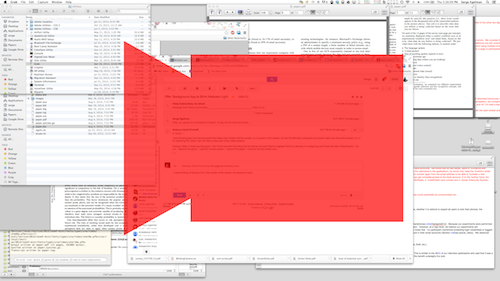
\includegraphics[width=3.4in]{redglyph-small.png}
\caption{Full screen image of the red camera glyph.}
\label{glyph}
\end{figure}

\subsection{Results}

We found that using the red camera glyph substantially increased the rate at which participants reported noticing the indicator. We also found that their understanding of what the warning indicated diminished, but not by a statistically significant amount. In this section, we compare the rates at which test group and control group participants noticed and understood the meanings of their respective indicators.

%\subsubsection{Noticing the Blinking LED}
% Of our 38 participants in the second set of experiments, 22 were female, and ages ranged from 18 to 59 years old ($\mu = 29.8$, $\sigma = 10.9$). Of the 38 participants, 9 were in the control group. In the control group, 6 were female, and ages ranged from 23 to 57 years old ($\mu = 35.0$, $\sigma = 12.8$). In the test group, 16 were female, and ages ranged from 18 to 59 years old ($\mu = 28.2$, $\sigma = 10.0$).

%When we asked during the exit survey whether anything unexpected had occurred during the computer-based task, the majority of test group participants did not report noticing the blinking LED light; none of the control group noticed the standard LED (see Table 10). Using Fisher's exact test we determined that the difference between the control group's rate of noticing the LED light and the test group's rate of the same was not statistically significant; (\textit{p} $=$ 0.5536; two-tailed).

%\begin {table}
%\begin{tabular}{lll}
 %            & Blinking LED & Control \\
%\hline
%noticed LED & 13.8\% (4 of 29) & 0\% (0 of 9) \\
%noticed nothing & 55.2\% (16 of 29) &  77.8\% (7 of 9) \\
%noticed something else & 31.0\% (9 of 29) & 22.2\% (2 of 9) \\
%\hline
%\end{tabular}
%\caption {Unprompted Responses, during Computer-Task: Blinking LED}
%\end {table}

%\begin {table}
%\begin{tabular}{lll}
 %            & Blinking LED & Control \\
%\hline
%noticed LED & 3.4\% (1 of 29) & 0\% (0 of 9) \\
%noticed nothing & 65.5\% (19 of 29) &  100\% (9 of 9) \\
%noticed something else & 31.0\% (9 of 29) & 0\% (0 of 9) \\
%\hline
%\end{tabular}
%\caption {Unprompted Responses, during Written Questionnaire: Blinking LED}
%\end {table}

%When asked the same question for the written questionnaire, the rate at which test group participants reported noticing the blinking LED light was lower; again none of the control group participants noticed their warning mechanism (see Table 11). Using Fisher's exact test we found that the difference between the control group's and the test group's rate of noticing was not statistically significant (\textit{p} $=$ 1.00; two-tailed).

%When prompted, the rate at which participants reported noticing the blinking LED improved, but only slightly; the majority of test group participants said nothing occurred during the computer task, and only 1 test group participant reported noticing the blinking LED in the written questionnaire (see Tables 12 and 13). For the control group, almost no one noticed the LED for both during the computer task and during the written questionnaire. Using Fisher's exact test we found that the difference between the control group's rate of reporting a light above the screen turning on and the test group's rate of the same for both during the computer-based task and the written questionnaire was not statistically significant:  (\textit{p} $=$ 0.4030; two-tailed) and (\textit{p} $=$ 1.00; two-tailed), respectively.

%\begin {table}
%\begin{tabular}{lll}
 %            & Blinking LED & Control \\
%\hline
%light & 27.6\% (8 of 29) & 11.1\% (1 of 9) \\
%recording & 37.9\% (11 of 29) &  11.1\% (1 of 9) \\
%something else & 13.8\% (4 of 29) & 11.1\% (1 of 9) \\
%nothing & 51.7\% (15 of 29) & 77.8\% (7 of 9) \\
%\hline
%\end{tabular}
%\caption {Prompted Responses, during Computer-Task: Blinking LED}
%\end {table}

%\begin {table}
%\begin{tabular}{lll}
 %            & Blinking LED & Control \\
%\hline
%light & 3.45\% (1 of 29) & 0\% (0 of 9) \\
%recording & 3.45\% (1 of 29) &  0\% (0 of 9) \\
%something else & 20.7\% (6 of 29) & 11.1\% (1 of 9) \\
%nothing & 79.3\% (23 of 29) & 88.9\% (8 of 9) \\
%\hline
%\end{tabular}
%\caption {Prompted Responses, during Written Questionnaire: Blinking LED}
%\end {table}

%As our preliminary results did not show signs of improvement using the blinking LED over the control group, we chose to focus our attention and resources on our second mitigation.

%\subsection{Understanding the Blinking LED}

%We used Fisher's exact test to see whether including the blinking improved participants' understanding of %the purpose of the LED. We found that for the control, 


%In order to assess whether, we tabulated the number of participants who, when prompted, reported only %that a light above the screen had turned on, vs. reporting that both a light above the screen had turned on, %and that the webcam had turned on. We found that for the computer-based task, 45.5\% (20 of 44) of the %participants only reported a light above the screen had turned on; for the written questionnaire, the %reporting rate was 40.0\% (2 of 5). These results indicate a clear problem with the LED as a warning %mechanism: even if users do notice the LED  turning on, a significant number of them do not understand %what that means. 

%the control group's rate of reporting the webcam began recording and the test group's rate of the same was %not statistically significant (\textit{p} $<$ 0.30; two-tailed). 

%the difference between the control group's rate of reporting the webcam began recording and the test %group's rate of the same was not statistically significant  (\textit{p} $=$ 1.00; two-tailed).
%

\subsubsection{Noticing the Red Camera Glyph}

We asked participants whether anything unexpected had occurred during the computer-based task or the written task.  We accepted any statement that reported the webcam turning on or the red camera glyph appearing as evidence that they noticed the red camera glyph. We observed that 65.9\% (29 of 44) of participants in the experimental group reported noticing the camera glyph appear (Table \ref{glyph-unprompted}). In contrast, only 16.2\% (6 of 37) of control group participants reported noticing the webcam LED.  This difference is statistically significant ($p<0.0001$; two-tailed Fisher's exact test), with a very large effect size ($\phi=0.500$).


%& n = 44 & n = 37 \\
%\textbf{Computer Task} : & & \\
%\MyIndent warning signal & 65.9\% (29 of 44) & 16.2\% (6 of 37) \\
%\MyIndent nothing & 34.1\% (15 of 44) &  70.3\% (26 of 37) \\
%\textbf{Written Questionnaire} : & & \\
%\MyIndent warning signal & 40.9\% (18 of 44)  & 2.7\% (1 of 37) \\
%\MyIndent nothing & 59.1\% (26 of 44) &  89.2\% (33 of 37) \\
%\caption {Unprompted Responses: Red Cam Glyph}

\begin {table}
%\small
\centering
\begin{tabular}{lll}
             & Noticed & \\
\hline
\textbf{Computer Task} & &  \\
\MyIndent Experimental & 65.9\% & n = 44 \\
\MyIndent Control & 16.2\% & n = 37 \\
\textbf{Written Task} & & \\
\MyIndent Experimental & 40.9\% & n = 44 \\
\MyIndent Control & 2.7\% & n = 37 \\
\hline
\end{tabular}
\caption {Unprompted responses: the number of participants who described noticing the indicator appear/turn on.}
\label{glyph-unprompted}
\end {table}

 %            & Red Cam Glyph & Control \\
%warning signal & 40.9\% (18 of 44)  & 2.7\% (1 of 37) \\
%nothing & 59.1\% (26 of 44) &  89.2\% (33 of 37) \\
%noticed something else & 0\% (0 of 44) & 8.1\% (3 of 37) \\
%\caption {Unprompted Responses, during Written Questionnaire: Red Cam Glyph}

When asked the same question for the written task, over 40\% of the experimental group participants reported noticing the red camera glyph, whereas only one participant in the control group reported noticing the webcam LED turn on (see Table \ref{glyph-unprompted}). This difference was also statistically significant ($p<0.0001$; two-tailed Fisher's exact test), with a very large effect size ($\phi=0.449$).

When prompted, participants saw the same seven options as in the first laboratory experiment, but with an added option: ``a red camera image appeared on the screen.'' When prompted, 93.2\% (41 of 44) of experimental group participants reported noticing the red camera glyph during the computer-based task (Table \ref{glyph-prompted}). For the control group, fewer than half reported noticing the webcam LED. This difference was statistically significant ($p<0.0001$; two-tailed Fisher's exact test), with a very large effect size ($\phi=0.568$).

%& n = 44 & n = 37 \\
%warning signal & 93.2\% (41 of 44) & 40.5\% (15 of 37)  \\
%recording & 25.0\% (11 of 44) &  37.8\% (14 of 37) \\
%nothing & 29.5\% & 83.8\% \\
%\textbf{Written Questionnaire} : & & \\
%warning signal & 59.1\% (26 of 44) & 5.41\% (2 of 37) \\
%recording & 18.2\% (8 of 44) & 5.41\% (2 of 37) \\
%something else & 18.2\% (8 of 44) & 13.5\% (5 of 37) \\
%nothing & 29.5\% (13 of 44) & 83.8\% (31 of 37) \\

\begin {table}
%\small
\centering
\begin{tabular}{llll}
             & Indicator & Recording & \\
\hline
\textbf{Computer Task} & & &  \\
\MyIndent Experimental & 93.2\% & 25.0\% &  n = 44 \\
\MyIndent Control & 40.5\% & 37.8\% & n = 37 \\
\textbf{Written Task} & & & \\
\MyIndent Experimental & 59.1\% & 18.2\% & n = 44 \\
\MyIndent Control & 5.41\% & 5.41\% & n = 37 \\
\hline
\end{tabular}
\caption {Prompted responses: number of participants who selected either that the indicator appeared or that the webcam began recording.}
\label{glyph-prompted}
\end {table}

%25.0\% (11 of 44) said that a light above the screen turned on

When asked the same question for the written task, over half of our participants in the experimental group reported noticing the red camera glyph, whereas only two control group participants reported noticing the webcam LED turn on (Table \ref{glyph-prompted}). This difference was statistically significant ($p<0.0001$; two-tailed Fisher's exact test), with a very large effect size ($\phi=0.562$).

We used McNemar's test to determine that participants were significantly more likely to notice the red camera glyph when performing the computer-based task than the written task, based on both the unprompted ($p=0.0003$; $\chi^2 = 13.067$) and prompted ($p=0.0026$; $\chi^2$ = 9.091) responses.  Using either measure, we observed relatively large effect sizes ($\phi_{unprompted} = 0.402$, $\phi_{prompted} = 0.335$), which indicates that participants were more likely to notice the red camera glyph while performing a task on the computer, rather than merely in its proximity.

%\% (9 of 44) said that a light above the screen turned on,

In all cases, the rate at which participants noticed the indicator was significantly better when viewing the red camera glyph than when viewing the standard webcam LED.

\subsubsection{Understanding the Red Camera Glyph}

We were curious to see whether or not using the red camera glyph as the indicator vs. the webcam LED changed the rate at which participants understood that the webcam was recording. When looking at the unprompted responses for the test group, of the participants who noticed the glyph, but did not explicitly state it was a camera, most reported seeing some combination of red blocks, shapes and symbols:

\begin{quotation}
\noindent {\it ``[I saw] a few red arrows or shapes flashed on the screen.''} (P2)\\

\noindent {\it ``[I saw] flashes of a faint red arrow across the screen.''} (P3)\\

%\noindent {\it ``There was a red shadow image that danced around at one point.''} (P14)\\

\noindent {\it ``...a couple red flashing symbols appeared on the screen.''} (P19)

%\noindent {\it ``[I saw] a few iterations of a red shape, in different sizes and places on the screen.''} (P39)\\

%\noindent {\it ``The screen was flashing as red.''} (P71)\\
\end{quotation}

We found that 25.0\% (11 of 44) of experimental group participants reported that the webcam began recording during the computer-based task, compared to 37.8\% (14 of 37) of participants in the control group (Table 5). For the written task, the corresponding rates were 18.2\% (8 of 44) and 5.41\% (2 of 37), respectively.

%For the test group for the computer-based task, we found that 73.2\% (30 of 41) of the participants who reported noticing the red camera glyph \textit{only} reported the glyph, and not also that the webcam had started recording. For the control group, the reporting rate was 30.0\% (3 of 15). In other words, the majority of participants may not have understood that the red camera glyph indicated that the webcam was recording; in contrast most participants seem to have understood the webcam LED. The difference between the test group's rate of understanding and the control group's rate of understanding is statistically significant (\textit{p} $<$ 0.0006; two-tailed), with a very large effect size (Cramer's \textit{V} = 0.4786).

%For the written questionnaire for the test group, the reporting rate was 69.2\% (18 of 26); for the control group the reporting rate was zero. The difference here is not statistically significant (\textit{p} $=$ 0.1190; two-tailed). 

%When looking at the unprompted responses for the test group, 32.1\% (9 of 28) of participants who reported noticing the red camera glyph appear to not have understood that the glyph was a camera. Of the participants who noticed the glyph but did not explicitly state it was a camera, most reported seeing some combination of red blocks, shapes and symbols:

In both cases, the difference was not statistically significant: ($p=0.236$, two-tailed Fisher's exact test) and ($p=0.101$, two-tailed Fisher's exact test) for the computer-based task and written task, respectively. These results seem to indicate that the number of participants who understood our warning mechanism was essentially the same as the number that understood the standard webcam LED.

The results of our experiment demonstrate that our red camera glyph indicator significantly outperformed the standard webcam LED in terms of participants' rate of noticing the indicator, with similar comprehension rates. In the next section, we analyze the results of our exit survey to see whether any correlations can be found between participants' previous experiences noticing their personal webcam turning on unexpectedly, and noticing the indicator in our experiments. 

\section{Exit Survey}

%In this section, we analyze the results of our exit survey to see whether any correlations can be found between various participants' behavior and attitudes, and noticing the webcam LED. In the remainder of this section, we detail the responses in the exit survey for the questions about participants' previously experiencing their personal webcam turning on unexpectedly, their security and privacy concerns, and their security behavior regarding their webcams.

In this section, we examine participants' previous experiences with having their personal webcams turn on unexpectedly, their security and privacy concerns, and their security behavior regarding their webcams, as gathered from our exit survey.

\subsection{Experienced Webcam Turning on Unexpectedly}

Of the 179 participants from our two lab experiments, 13.4\% (24 of 179) had experienced a webcam turn on unexpectedly some time in the past (i.e., prior to this study), 79.9\% (143 of 179) had not, and the remaining 6.70\% (12 of 179) were unsure if this had ever happened. 

%If we removed those participants who had their webcam turn on unexpectedly because of some clear human error on their part (i.e. accidently clicking on the FaceTime icon thinking it was some other program), the number dropped to 10.6\% (19 of 179).

%CT noticing: -2

We compared participants' prior experiences with their behaviors in the laboratory, excluding those who were unsure whether their webcams had ever turned on unexpectedly. Of the 24 who claimed to have experienced it in the past, when prompted, 20.8\% (5 of 24) reported noticing the indicator during the computer-based task; of the 143 who had not experienced it, 56.6\% (81 of 143) reported the same. This difference was statistically significant ($p<0.0025$; two-tailed Fisher's exact test) with a medium effect size ($\phi=0.251$). For the written task, 8.33\% (2 of 24) reported noticing the indicator; of the 143, 16.8\% (24 of 143) reported the same. However, this difference was not statistically significant.

In other words, for the computer-based task, it seems that those who had prior experiences with webcams turning on unexpectedly were {\it less} likely to notice it happen in the laboratory, which seems counterintuitive. It seems likely that some other confounding factor is in effect here. It could be the case that previous victims have become accustomed to the protection their personal security measures provide, and as a result do not pay as much attention to the webcam indicator. We found that 29.2\% (7 of 24) of participants who have previously noticed their webcams turn on unexpectedly claim to now cover the camera lens of their home computer/laptop when not in use, as compared to 9.79\% (14 of 143) of those who have not. The difference was statistically significant ($p=0.0157$, two-tailed Fisher's exact test) with a medium effect size ($\phi=0.2050$), though this effect may not be statistically significant upon correcting for multiple testing (e.g., using the Bonferroni correction).

\subsection{Security/Privacy Concerns}

%As part of our exit survey, we asked the participants to state any and all reasons why their webcam might begin recording unexpectedly. 
%Most participants offered multiple explanations; we classified them into two groups: ``low risk perception'' and ``high risk perception'' explanations. The low risk perception explanations consisted of the following:

%\begin{packed_item}
%\item normal computer activity
%\item computer error
%\item human error
%\end{packed_item}

%The high risk explanations were:

%\begin{packed_item}
%\item virus
%\item spying
%\item hacking
%\end{packed_item}

%Of our 179 participants, 15.1\% (27 of 179) provided only answers from the low risk group; 45.3\% (81 of 179) provided only answers from the high risk group. 

%Of the 27, 66.7\% (18 of 27) when prompted reported noticing the indicator during the computer-based task portion of the lab experiment; of the 81, 59.3\% (48 of 81) reported noticing. The difference between these is not statistically significant (\textit{p} $=$ 0.6468; two-tailed). For the written questionnaire, 29.6\% (8 of 27) of the former group reported noticing the indicator, while 19.8\% (16 of 81) of the latter group reported noticing. The difference between these is not statistically significant (\textit{p} $=$ 0.4237; two-tailed). 

%In other words, in both the computer-based task case and the written questionnaire, we were unable to reject the null hypothesis that participants' risk perceptions have no demonstrable impact on whether they notice the indicators.

% (see Table 11). Based on their responses, many participants seem to think that this might indicate the presence of an intruder; ``hacking'' was the most popular explanation. Some participants referenced stories they had heard and articles they had read when giving their explanation:

%\begin {table}
%\centering
%\begin{tabular}{ll}
%normal computer activity & 7.37\% (16 of 217) \\
%don't know & 13.4\% (29 of 217) \\
%virus & 18.4\% (40 of 217) \\
%computer error & 20.3\% (44 of 217) \\
%spying & 26.3\% (57 of 217) \\
%human error & 28.6\% (62 of 217) \\
%hacking & 41.9\% (91 of 217) \\
%\hline
%\end{tabular}
%\caption {What might cause your webcam to begin recording unexpectedly?}
%\end {table}

%\begin{quotation}
%\noindent {\it ``I read an article about a guy who took over people's computers remotely and recorded %them...''} (P51)\\

%\noindent {\it ``One hears that it could be remote manipulation by the NSA, FBI, DHS, et al to spy on you...''} (P84)\\

%\noindent {\it ``I've heard people can tap into your webcam via some sort of remote control but I don't know if thats true. If it is that is insanely creepy.''} (P102)\\

%\noindent {\it ``I ... read once that a school did this on borrowed laptops. I would assume I was being hacked.''} (P115)\\

%\noindent {\it ``I have heard that people can just start recording... It kind of freaks me out.''} (P170)\\

%\end{quotation}



%Almost half of the participants, 41.5\% (90 of 217) offered multiple explanations. When dividing participants' responses into those that involved an intruder and those that did not, we found that 41.0\% (89 of 217) gave a response that involved an intruder, i.e. consisted of some combination of ``hacking'', ``spying'', and ``virus'', vs. 11.5\% (25 of 217) who gave a response that did not, i.e. consisting of some combination of ``human error'', ``computer error'', and ``normal computer activity''. These results seem to indicate that when it comes to their webcam unexpectedly turning on, participants are most suspicious of outside intruders. 


%The 5 most popular combinations can be seen in Table 19. 
%\begin {table}
%\centering
%\begin{tabular}{ll}
%spying, human error & 6.67\% (6 of 90) \\
%spying, computer error & 7.78\% (7 of 90) \\
%hacking, computer error & 8.89\% (8 of 90) \\
%hacking, spying & 11.1\% (10 of 90) \\
%hacking, human error & 17.8\% (16 of 90) \\
%\hline
%\end{tabular}
%\caption {Multiple Explanations}
%\end {table}

%We saw something similar when looking at participants' security and privacy concerns. 

%; we classified these into ``high concern'', ``medium concern'' and ``low concern.'' The low concern options were:
%
%\begin{packed_item}
%\item don't care
%\item nothing
%\end{packed_item}
%
%The medium concern options were:
%
%\begin{packed_item}
%\item violation of privacy
%\item embarrassment
%\item negative feelings
%\item unspecified negative result
%\end{packed_item}
%
%The high concern options were: 
%
%\begin{packed_item}
%\item compromise reputation
%\item confidential information leakage
%\end{packed_item}

When asked to state any and all possible consequences if the webcam on their home computer/laptop unexpectedly recorded them and the video became public, most participants offered multiple responses. The most frequent response was ``violation of privacy.'' As one participant poignantly stated:
\begin{quotation}
\noindent {\it ``I would look foolish, I'm sure. People would see me at my best and at my worst. They would see my daughter and husband when they weren't expecting it. They would see us in our most intimate moments. I would be devastated that our privacy was violated so completely. It would be like someone broke into our home and stole our secrets.''} (P90)
\end{quotation}

Many participants stated concern over intimate moments being made public:
\begin{quotation}
%\noindent {\it ``Well, I might show up on a porn site...''} (P3)\\

%\noindent {\it ``They might see me jerkin' the gurken, but probably not.''} (P34)\\

%\noindent {\it ``Ack. OK. I care I care. People would have pictures of me, mainly eating and studying, but perhaps getting undressed as well.''} (P38)\\

%\noindent {\it ``They would see me naked... I'd be mortified.''} (P63)\\

%\noindent {\it ``Probably end up on a porn site...''} (P98)\\

\noindent {\it ``There would be a sex video online somewhere, I would be seen completely naked from changing out of the shower, or I would be sleeping in my bed.''} (P127)\\

\noindent {\it ``I'd feel really violated, I mean sometimes I'm sitting in front of my computer naked, or smoking weed, and I'd be really uncomfortable with video like that becoming public.''} (P150)\\

\noindent {\it ``The camera might... record me masturbating.''} (P156)\\

\noindent {\it ``I live in a studio with my boyfriend, so the video might end up on a porn site.''} (P188)

\end{quotation}

A smaller subset of participants were more worried about what other data/information a hacker might be able to gain access to while spying on them:

\begin{quotation}
%\noindent {\it ``It could ... give clues (from my background) as to where my residence is.''} (P6)\\

\noindent {\it ``Not sure. Possibly home burglary because they can see what's in the house.''} (P10)\\

\noindent {\it ``...identity theft or loss of money.''} (P34)\\

%\noindent {\it ``...every electronic thing I have on my computer.''} (P48)\\

\noindent {\it ``I'm more concerned about this being a warning sign that someone has access to all the information on my computer...''} (P51)

\end{quotation}

%Of our 179 participants, 30.2\% (54 of 179) provided only answers from the low concern group; 27.4\% (49 of 179) provided at least one answer from the high concern group, and none from the low concern group. 

%Of those 54 low-concern participants, 48.1\% (26 of 54) when prompted reported noticing the indicator during the computer-based task portion of the lab experiment; of the 49 high-concern participants, 57.1\% (28 of 49) reported noticing. The difference between these is not statistically significant (\textit{p} $=$ 0.4751; two-tailed). For the written questionnaire, 13.0\% (7 of 54) of low-concern participants reported noticing the indicator;  14.3\% (7 of 49) of high-risk participants reported noticing. The difference between these is not statistically significant (\textit{p} $=$ 0.9203; two-tailed). 

%In other words, in both the computer-based task case and the written questionnaire, we were unable to reject the null hypothesis that participants' level of security and privacy concerns have no demonstrable impact on whether they notice the indicators.

%\subsection{Security and Privacy Concerns}

%In order to gauge where participants' privacy and security concerns lay, we asked participants to select their level of concern if the webcam on their home computer or laptop began to unexpectedly record, and the severity of the consequences if this video became public (see Tables 19 and 20). While the majority of participants stated that they would be extremely concerned, only 15\% of participants believed there would be severe consequences: most participants believed there would be moderate to no consequences.


%\begin {table}
%\centering
%\begin{tabular}{ll}
%Unconcerned (1) & 2.30\% (5 of 217) \\
%Slightly Concerned (2) & 6.91\% (15 of 217) \\
%Somewhat Concerned (3) & 10.6\% (23 of 217) \\
%Moderately Concerned (4) & 19.4\% (42 of 217) \\
%Extremely Concerned (5) & 59.4\% (129 of 217) \\
%\hline
%\end{tabular}
%\caption {How concerned would you be if home webcam began recording unexpectedly}
%\end {table}

%\begin {table}
%\centering
%\begin{tabular}{ll}
%No Consequences (1) & 13.4\% (29 of 217) \\
%Minor Consequences (2) & 24.9\% (54 of 217) \\
%Moderate Consequences (3) & 28.1\% (61 of 217) \\
%Heavy Consequences (4) & 18.4\% (40 of 217) \\
%Severe Consequences (5) & 15.2\% (33 of 217) \\
%\hline
%\end{tabular}
%\caption {If home webcam recorded unexpectedly and that video became public, how serious would the %consequences be}
%\end {table}


%\begin {table}
%\centering
%\begin{tabular}{ll}
%don't know & 3.69\% (8 of 217) \\
%don't care & 5.07\% (11 of 217) \\
%compromise reputation & 5.53\% (12 of 217) \\
%confidential information leakage & 6.91\% (15 of 217) \\
%unspecified negative result & 6.91\% (15 of 217) \\
%negative feelings & 9.68\% (21 of 217) \\
%nothing & 26.3\% (57 of 217) \\
%embarrassment & 28.1\% (61 of 217) \\
%violation of privacy & 39.6\% (86 of 217) \\
%\hline
%\end{tabular}
%\caption {Possible consequences if home webcam unexpectedly recorded you and the video became public}
%\end {table}

%When asked to state the potential consequences if such a video were to become public, the most frequent %response was ``violation of privacy''. As one participant poingnantly stated:

%\begin{quotation}
%\noindent {\it ``I would look foolish, I'm sure. People would see me at my best and at my worst. They would %see my daughter and husband when they weren't expecting it. They would see us in our most intimate %moments. I would be devastated that our privacy was violated so completely. It would be like someone %broke into our home and stole our secrets.''} (P90)\\
%\end{quotation}

%Many participants stated concern over intimate moments being made public:

%\begin{quotation}
%\noindent {\it ``Well, I might show up on a porn site...''} (P3)\\

%\noindent {\it ``They might see me jerkin' the gurken, but probably not.''} (P34)\\

%\noindent {\it ``Ack. OK. I care I care. People would have pictures of me, mainly eating and studying, but perhaps getting undressed as well.''} (P38)\\

%\noindent {\it ``They would see me naked... I'd be mortified.''} (P63)\\

%\noindent {\it ``Probably end up on a porn site...''} (P98)\\

%\noindent {\it ``There would be a sex video online somewhere, I would be seen completely naked from changing out of the shower, or I would be sleeping in my bed.''} (P127)\\

%\noindent {\it ``I'd feel really violated, I mean sometimes I'm sitting in front of my computer naked, or smoking weed, and I'd be really uncomfortable with video like that becoming public.''} (P150)\\

%\noindent {\it ``The camera might... record me masturbating.''} (P156)\\

%\noindent {\it ``I live in a studio with my boyfriend, so the video might end up on a porn site.''} (P188)\\

%\end{quotation}

%A smaller subset of participants were more worried about what other data/information a hacker might be able to gain access to while spying on them:

%\begin{quotation}
%\noindent {\it ``It could ... give clues (from my background) as to where my residence is.''} (P6)\\

%\noindent {\it ``Not sure. Possibly home burglary because they can see what's in the house.''} (P10)\\

%\noindent {\it ``...identity theft or loss of money.''} (P34)\\

%\noindent {\it ``...every electronic thing I have on my computer.''} (P48)\\

%\noindent {\it ``I'm more concerned about this being a warning sign that someone has access to all the information on my computer...''} (P51)\\

%\end{quotation}

%When looking at just the participants who stated they would be extremely concerned, 13.2\% (17 of 129) believed there would be no consequences. This seemed strange; however, when looking at the free-form responses, we found that most of these participants did not use their computers/laptops in compromising locations or leave them turned on for extended periods of time:

%\begin{quotation}
%\noindent {\it ``It wouldn't concern me, as my computer is closed 95\% of the time...''} (P8)\\

%\noindent {\it ``There's nothing in my environment that would generate interest.''} (P11)\\

%\noindent {\it ``... I turn it off when I'm not using it, so there would be little to see except some book shelves and a lamp.''} (P25)\\

%\noindent {\it ``Nothing much, it would probably just see my kitchen.''} (P41)\\

%\noindent {\it ``I use my laptop for work at home so whatever video goes public would just capture - at worst - my faces of frustration and concentration.''} (P61)\\

%\end{quotation}

%It seems that to some participants, the idea of an intruder accessing this private footage is more concerning than the actual consequences that may result, as they have confidence in their computer usage habits.

%Overall, our survey data suggests that most participants are more concerned about privacy violations than security violations in regards to their webcams: e.g. footage of intimate moments being released vs. burglary, both physical and electronic. Additionally, although most people express extreme concern in the circumstance of a webcam intruder, there is a significant minority that is confident they will not experience any consequences, due to their computer usage habits.

%\begin{quotation}

%\noindent {\it ``I'd be discovered by Hollywood and would have to fight off the legion of fans. (LOL). %Seriously though, people would rather watch grass grow compared to what I do in front of my computer.''} %(P13)\\

%\noindent {\it ``The world might see me without makeup and in clothes that I would not wear outside of %the home (clothes that expose body parts that I would not want the general public to see). Also, the world %might see my cats, which is much better than seeing me in an indecent state.''} (P32)\\

%\noindent {\it ``I often use my computer in bed. I don't think I have ever had it opened in a way the would %record me doing anything sexual. I doubt anyone would really care enough to watch a video of me in a bra %typing.''} (P35)\\
%\end{quotation}

\subsection{Security Behavior}

%We asked participants whether they currently covered the camera lens of their home computer/laptop webcam with any kind of tape or other occluding material. 13.4\% (24 of 179) of our participants do so; 86.6\% (155 of 179) do not. 

%Of those 24 who do cover their camera lens, 66.7\% (16 of 24) when prompted reported noticing the indicator during the computer-based task portion of the lab experiment; of the 155 who do not, 54.2\% (84 of 155) reported noticing. The difference between these is not statistically significant (\textit{p} $=$ 0.3566; two-tailed). For the written questionnaire, 16.7\% (4 of 24) lens-covering participants reported noticing the indicator; 18.7\% (29 of 155) non-lens-covering participants reported noticing. The difference between these is not statistically significant (\textit{p} $=$ 1.0; two-tailed). 

%In other words, in both the computer-based task case and the written questionnaire, we were unable to reject the null hypothesis that participants' covering of the lens on their personal webcam has no demonstrable impact on whether they notice the indicators.

%\begin {table}
%\centering
%\begin{tabular}{ll}
%yes, for some machines & 3.69\% (8 of 217) \\
%used to, no longer do & 4.61\% (10 of 217) \\
%yes & 10.1\% (22 of 217) \\
%considered it, but not done & 28.1\% (61 of 217) \\
%no & 53.0\% (115 of 217) \\
%\hline
%\end{tabular}
%\caption {Do you cover your webcam camera lens?}
%\end {table}

%; we classified these into ``highly secure'', ``medium secure'' and ``low secure.'' The low secure options were:
%
%\begin{packed_item}
%\item nothing
%\end{packed_item}
%
%The medium secure options were:
%
%\begin{packed_item}
%\item turn webcam off
%\item turn computer off
%\item seek outside help
%\item cover camera lens
%\item unspecified self fix
%\item virus scan
%\end{packed_item}
%
%The highly secure options were: 
%
%\begin{packed_item}
%\item get new device
%\end{packed_item}

When asked to state what participants would do if the webcam on their home computer/laptop began recording unexpectedly, the most frequent response was ``cover the camera lens,'' followed closely by ``seek outside help.'' Almost every participant stated that they would try some way to ``fix'' the problem, even if they could not state exactly what steps they would take:

\begin{quotation}
\noindent {\it ``I would try to determine the cause of the unexpected recording and then take measures to prevent it from happening in the future.''} (P21)\\

\noindent {\it ``I would investigate and see if I could stop [it]...''} (P78)\\

\noindent {\it ``I would try to figure out how to stop it from doing it and try to figure out how to not let that happen again.''} (P188)

\end{quotation}


Some participants stated they would resort to more extreme measures:

\begin{quotation}
\noindent {\it ``Scan, and if necessary, bomb the harddrive.''} (P17)\\

\noindent {\it ``Disconnect it when not in use, possibly destroy it.''} (P44)\\

\noindent {\it ``Throw it out the window...''} (P63)

\end{quotation}

It is clear to see from these responses that participants value their security and privacy, and are troubled by the thought of someone watching them without their permission.

%Of our 179 participants, 3.35\% (6 of 179) only provided answers from the low secure group; 5.59\% (10 of 179) provided at least one answer from the highly secure group, and none from the low secure group. 

%Of those 6 low secure participants, 83.3\% (5 of 6) when prompted reported noticing the indicator during the computer-based task portion of the lab experiment; of the 10 highly secure, 40.0\% (4 of 10) reported noticing. The difference between these is not statistically significant (\textit{p} $=$ 0.1451; two-tailed). For the written questionnaire, 50.0\% (3 of 6) low secure participants reported noticing the indicator; 30.0\% (3 of 10) highly secure participants reported noticing. The difference between these is not statistically significant (\textit{p} $=$ 0.6066; two-tailed). 

%In other words, in both the computer-based task case and the written questionnaire, we were unable to reject the null hypothesis that participants' response to their webcam light turning on unexpectedly have no demonstrable impact on whether they notice the indicators.

%\begin {table}
%\centering
%\begin{tabular}{ll}
%nothing & 4.15\% (9 of 217) \\
%get new device & 4.61\% (10 of 217) \\
%virus scan & 8.29\% (18 of 217) \\
%turn webcam off & 18.9\% (41 of 217) \\
%turn computer off & 27.2\% (59 of 217) \\
%self fix & 27.2\% (59 of 217) \\
%seek outside help & 28.1\% (61 of 217) \\
%cover camera lens & 33.2\% (72 of 217) \\
%\hline
%\end{tabular}
%\caption {What would you do if your webcam began recording unexpectedly?}
%\end {table}

%Overall, from these results it seems that participants believe they would be motivated to take active measures to behave securely given one bad experience. However, we found that this may not actually be the case. Of our 217 participants, 32 had experienced the webcam on their home computer/laptop turning on unexpectedly some time in the past, 168 had not, and the remaining 17 were unsure if this had ever happened. Of those 32, 21.9\%  (7 of 32) reported that they currently covered their camera lens when not in use; of the 168, 10.1\% (17 of 168) reported the same. We found that the difference between these two rates is not statistically significant (\textit{p} $=$ 0.1725; two-tailed).

\section{Limitations}
After completing our experiments, we realized that by not randomizing the order in which the computer task versus the written task was performed, we could not guarantee that there was no learning or habituation effect. Although this was an unfortunate oversight, we found that for everything but the mitigation experimental group, it had no observable effect on our results. We performed Phi correlations between the rates of noticing the indicators between the two tasks and found no statistically significant correlations for the first laboratory experiment ($p<0.49$, $\phi=0.07$) or for the followup mitigation experiment in the control group ($p<0.083$, and $\phi=0.29$). For the experimental group (i.e., the red camera glyph), we found a potentially significant correlation ($p<0.029$, $\phi=0.33$), though upon correcting for multiple testing, it is unlikely to remain statistically significant. Given these results, there is no evidence to suggest that this oversight impacted our conclusion regarding the utility of the webcam LED as a warning mechanism, or the improvement gained by the red glyph.

\section{Discussion}
In this section, we discuss the space of future mitigation research as we see it, as well as more sophisticated attacks.

\subsection{Mitigations}

While we found the red camera glyph, taken as a whole, to be significantly more effective than the status quo, it is by no means the only solution (or necessarily the best). More work is needed to show how each change contributed individually, as the red camera glyph differed in size, color, and movement, as compared to the existing webcam LED. More broadly speaking, more work is needed to explore other potential design improvements. We see two main categories of study which remain to be explored in regard to webcam indicators, as well as privacy indicators in general:

\begin{packed_enum}
\item Designing indicators that users will notice
\item Improving user understanding of the indicators
\end{packed_enum}

\subsubsection{Noticeable Indicators}

We see two main classes of potential indicators for the webcam, namely hardware-based and software-based indicators. Hardware-based solutions are preferable, as they prevent a hacker who has used a root exploit to gain control of the machine from accessing the webcam without triggering the indicator. Existing webcam LED indicators are typically implemented in hardware. For our experiments, we implemented the red camera glyph in software, which means that an attacker with root access could disable it. Any real-life implementation of the red camera glyph as an indicator would need to be implemented in hardware, like the standard webcam LED currently is.

One natural way to expand on the current webcam LED is to have it flash/blink, rather than hold steady. The most basic set up would be to have the webcam LED blinking constantly throughout the duration of the recording, though this might be distracting or irritating for users. Alternatively, the LED could blink when the webcam is first turned on, in order to draw the user's attention to it immediately, and after some amount of time, it could return to a steady light. The LED could also blink intermittently throughout the recording; this might be useful in drawing the user's attention to the LED even when the user did not initially notice it.

In a pilot experiment, we explored whether simply blinking the webcam LED would be sufficient. While blinking the LED did not yield significantly improved results over the control condition, %(n = 29 in the blinking condition, n = 9 in the control condition; \textit{p} $=$ 0.4030; two-tailed during the computer-based task and \textit{p} $=$ 1.00; two-tailed) during the written task),
that may have been because the frequency of blinking was only 0.5 Hz. We were not able to increase this speed due to hardware limitations. It seems possible that with a faster blinking speed, more users might notice the LED.

Exploring a larger variety of computer-based tasks could also be worthwhile. Determining whether users are more likely to notice the webcam indicator when performing tasks that are menial and/or automatic vs. active and require conscious attention could allow researchers to design indicators that have a varying signal size based on task. For example, if the webcam turned on while the user was performing a menial or automatic task, the indicator signal would be smaller; if it turned on while the user was performing a task requiring conscious attention and focus, the signal would be larger.

Another challenge is to to help users notice the indicator when they are not using their computers, but are in the same room as their computers. This challenge is especially important because it includes the scenario of when a person is in a compromising or intimate situation. A brighter webcam LED might help in this circumstance (e.g., a flash LED). Using an audio signal could also be helpful in this scenario, although not for people who regularly leave their headphones plugged in, mute their computer, or have hearing problems.

%A brighter LED light might also improve the rate at which users notice the indicator. LED indicators at varying levels of brightness could be investigated, possibly mimicking something similar to the ``flash'' that currently exists on standard cameras.

%Indicators should be noticeable in a variety of situations. We saw in our initial experiment that there was little noticeable effect (among the sample size) of computer-based task on whether participants noticed the LED. We believe it is equally important to explore a variety of non computer-based tasks, including those tasks where the participant is present in the same room as the computer, but is not necessarily sitting in front of the computer. This would more realistically replicate the real-life scenarios where a person is in a compromising or intimate situation.

\subsubsection{Improving Understanding}
It is critically important for people to comprehend what the warning signal means: without understanding, the indicator is useless. One possibility for improving comprehension would be to display a one-time-only explanation of the warning that appears the first time a person uses the webcam, and never again. This solution would not be dependent on a user's prior knowledge. However, it is unclear whether or not users would actually pay attention to the explanation. Given that current users are not used to a message appearing when they turn their webcams on, it is possible that users may automatically close it without paying attention, or even believe the message indicates the presence of malware on their machine.

Over time, people may come to learn the meaning of a new indicator such as our red camera glyph, simply because it always appears each time the webcam is in use. However, even time and experience are not a perfect solution: people have used the presence of a light as an indicator that video is recording for ages, and yet people still have confusion as to what exactly the webcam LED indicates. One possible alternative is to change the form of the webcam LED light; rather than having a small circle of light, the LED could be designed to emit light in the shape of a video camera. It is possible that the combination of the traditional LED light and the video camera shape could fix what time and experience have not.

\subsection{Sophisticated Attacks}

There are a number of ways in which attackers could attempt to spy on users through their webcams without the users realizing. One natural method would be to distract users from looking in the direction of the webcam LED when the webcam turns on, possibly by drawing their eye to somewhere else on the screen with a pop-up or some other distraction. Other techniques could use social engineering: an attacker could implement a false webcam driver update message that appears whenever he turns on the victim's webcam. The intention of the message would be to lull the user into a false sense of security, so even if she notices that the webcam is on and recording, she believes it is part of the update process.

Attackers could also use other features to infer when users are away from their computers, and are less likely to notice the webcam LED turning on. In the most trivial scenario, an attacker could wait until there is no activity on the computer to turn the webcam on. This could get more complex: a clever attacker could learn his victim's schedule and habits of computer usage to learn the optimal time to turn the webcam on. 

An attacker could potentially pick up this kind of information by remotely turning on the microphone. This sensor currently has absolutely no indicator for when it is turned on. This is a very serious concern, given the security and privacy implications of a malicious attacker listening in on a user's daily life and activities.

%\subsection{Limitations and Flaws}
%In our first mitigation, the blinking LED, due to hardware limitations we were not able to increase the speed of blinking beyond 0.5 Hz. It is possible that if we had been able to increase the blinking speed, more participants would have noticed the LED. 

%We found ourselves unable to confirm for the written quesionnaire task whether making eye contact with the camera correlated with self-reporting noticing the LED. It is possible that as a result the rate of noticing the warning mechanism, when participants were prompted for the written questionnaire, is artificially inflated. This seems unlikely, however, as the difference between the unprompted reponses and the prompted responses is minimal, and in almost all cases not statistically significant. The only case in which it is statistically significant is during the comptuer-based task for the red camera glyph (\textit{p} $<$ 0.003; two-tailed). 

%Even if the prompted response values are inflated, however, the unprompted responses alone overwhelmingly demonstrate our key claims that 1) the standard LED light is not an effective warning mechanism and 2) the red camera glyph demonstrates a significant improvement. When unprompted, only 16.2\% (6 of 37) of the control group reported noticing the LED during the computer-based task while 65.9\% (29 of 44) of the test group report the same; during the written questionnaire the rates were only 2.7\% (1 of 37) for the control and 40.9\% (18 of 44) for the test group.

%Although not necessarily a limitation of our current work, it is important to note that any real-life implementation of the red camera glyph as an indicator would need to be implemented in hardware, like the standard LED light currently is. Otherwise, this warning mechanism could be turned off remotely.

%\subsubsection{Improving Understanding}
%It is critically important for people to comprehend what the warning signal means: without understanding, regardless of whether or not people notice it the warning will not be successful. For both the traditional LED light and our red camera glyph mitigation mechanism, comprehension was not ideal, dipping as low as 26.8\% (11 of 41) for our red camera glyph mitigation.

%While this is a problem, it is not surprising: participants have no previous experience associating this particular stimulus with the webcam turning on. Given time and experience with the new warning mechanism, it seems likely that the comprehension rate will naturally increase. However, even time and experience are not a perfect solution: people have used the presence of a light as an indicator that video is recording since video recording was invented, and yet people still have confusion as to what exactly the LED light means. 

%One potential solution could be to include an explanation of the warning that appears the first time a person uses the webcam, and never again. This would allow for the user to be immediately made aware of the meaning, without depending upon any prior knowledge the user may or may not have. Another potential solution is to change the form of the LED light; rather than having a small circle of light, the LED could be designed to emit light in the shape of a video camera. It is possible that the combination of the traditional LED light and the video camera shape could fix what time and experience have not.

%\subsection{Future Work}

%There are several other potential mitigations that can be explored. If we can overcome the hardware limitations, it would be worthwhile to explore whether a faster blinking LED improved the rate of participants noticing the LED. Along that same vein, we could explore the effect a consistently brighter LED has, or a LED that flashes once very brightly then returns to the normal brightness. Additionally, experimenting with various potential ways to improve peoples' understanding of the warning mechanism would be a step in the right direction towards buiding an effective and highly-performing warning system.

%We also want to explore a larger variety of non computer-based tasks, including those tasks where the participant is present in the same room as the computer, but is not sitting in front of the computer. This would more realistically replicate the real-life scenarios where a person is in a compromising or intimate situation.

%We also would be interested in exploring in more depth what motivation a user would need to take simple steps to secure their webcam, such as covering the webcam camera lens when not actively using the camera.

\section{Conclusion}
We demonstrated that the current webcam LED is not effective as an indicator to communicate when the webcam is recording. We created our own indicator which significantly improved the rate at which participants noticed it, both during computer-based tasks and for non-computer-based tasks, without significantly decreasing their understanding. We analyzed our participants' previous experience with the webcam on their personal computer/laptop turning on unexpectedly, finding that this previous experience inversely correlated to noticing the webcam LED in our experiments. Based on our experimental results, we offer an initial step towards designing better webcam indicators for user. Finally, we outline the space of future mitigation research as we see it, to make sure users both notice and understand future privacy indicators.

%We demonstrated that the current LED light warning mechanism is not effective. We created our own warning mechanism which significantly improved the rate at which participants noticed the warning, both for computer-based tasks and for non computer-based tasks. We analyzed our participants' risk perceptions, security and privacy concerns and behavior regarding their webcams, finding that for the most part participants are aware and suspicious of the possibility of outside intruders accessing their webcams, more concerned about privacy violations than security violations, and not necessarily motivated to ensure webcam security. Based on these experiments, we offer a first step towards designing better warning mechanisms for users, as well as recognizing future work needed to make sure users both notice and understand the warning.

%\section{Acknowledgements}
%This work was made possible by Intel through the ISTC for Secure Computing, NSF award number %CNS-1318680, NSF award number CNS-1018924, and the and the AFOSR under MURI award %FA9550-12-1-0040.

% REFERENCES FORMAT
% References must be the same font size as other body text.

\section{Acknowledgements}

This work was supported by the Intel Science and Technology Center for Secure Computing (ISTC-SC), NSF under award CNS-1318680, and AFOSR under MURI award FA9550-12-1-0040. We would like to thank Vitaly Dubnovitsky for assistance implementing the webcam glyph.


%\raggedright
%\sloppy
\bibliographystyle{acm-sigchi}
\bibliography{sample}

\end{document}
